\documentclass[aspectratio=169]{beamer}

\usepackage{calc}
\usepackage{graphicx}
\usepackage{mathtools}
\usepackage{siunitx}
\usepackage{xcolor}

\graphicspath{{./images}}
\setbeamertemplate{navigation symbols}{}

\author{Chris Doble}
\date{}
\subtitle{Building a GPS receiver from scratch}
\title{Part 6: Tracking}
\usetheme{Madrid}

% Show the topics frame at the start of each section
\AtBeginSection[]
{
  \begin{frame}
    \frametitle{Topics}
    \tableofcontents[currentsection, subsubsectionstyle=hide]
  \end{frame}
}

% Show the topics frame at the start of each subsection
\AtBeginSubsection[]
{
  \begin{frame}
    \frametitle{Topics}
    \tableofcontents[currentsection, currentsubsection, subsubsectionstyle=hide]
  \end{frame}
}

\begin{document}

\frame{\titlepage}

\begin{frame}
    \frametitle{Goals}

    \begin{itemize}
        \item<2-> Track signal parameters over time
        
        \begin{itemize}
            \item<3-> Carrier wave frequency shift
            
            \item<4-> Carrier wave phase
            
            \item<5-> PRN code phase
        \end{itemize}

        \item<6-> Decode fragments of navigation message bits
        
        \begin{itemize}
            \item<7-> $\qty{1}{ms}$ samples $\Leftrightarrow$ 1 PRN code $\Leftrightarrow$ $1/20$ navigation message bit
        \end{itemize}

        \item<8-> Count PRN codes
        
        \begin{itemize}
            \item<9-> Required to calculate the signal transmission time
        \end{itemize}
    \end{itemize}
\end{frame}

\begin{frame}
    \frametitle{Topics}

    \tableofcontents
\end{frame}

\section{Carrier wipeoff}

\begin{frame}
    \frametitle{Carrier wipeoff}

    \centering
    \raisebox{0.66cm}{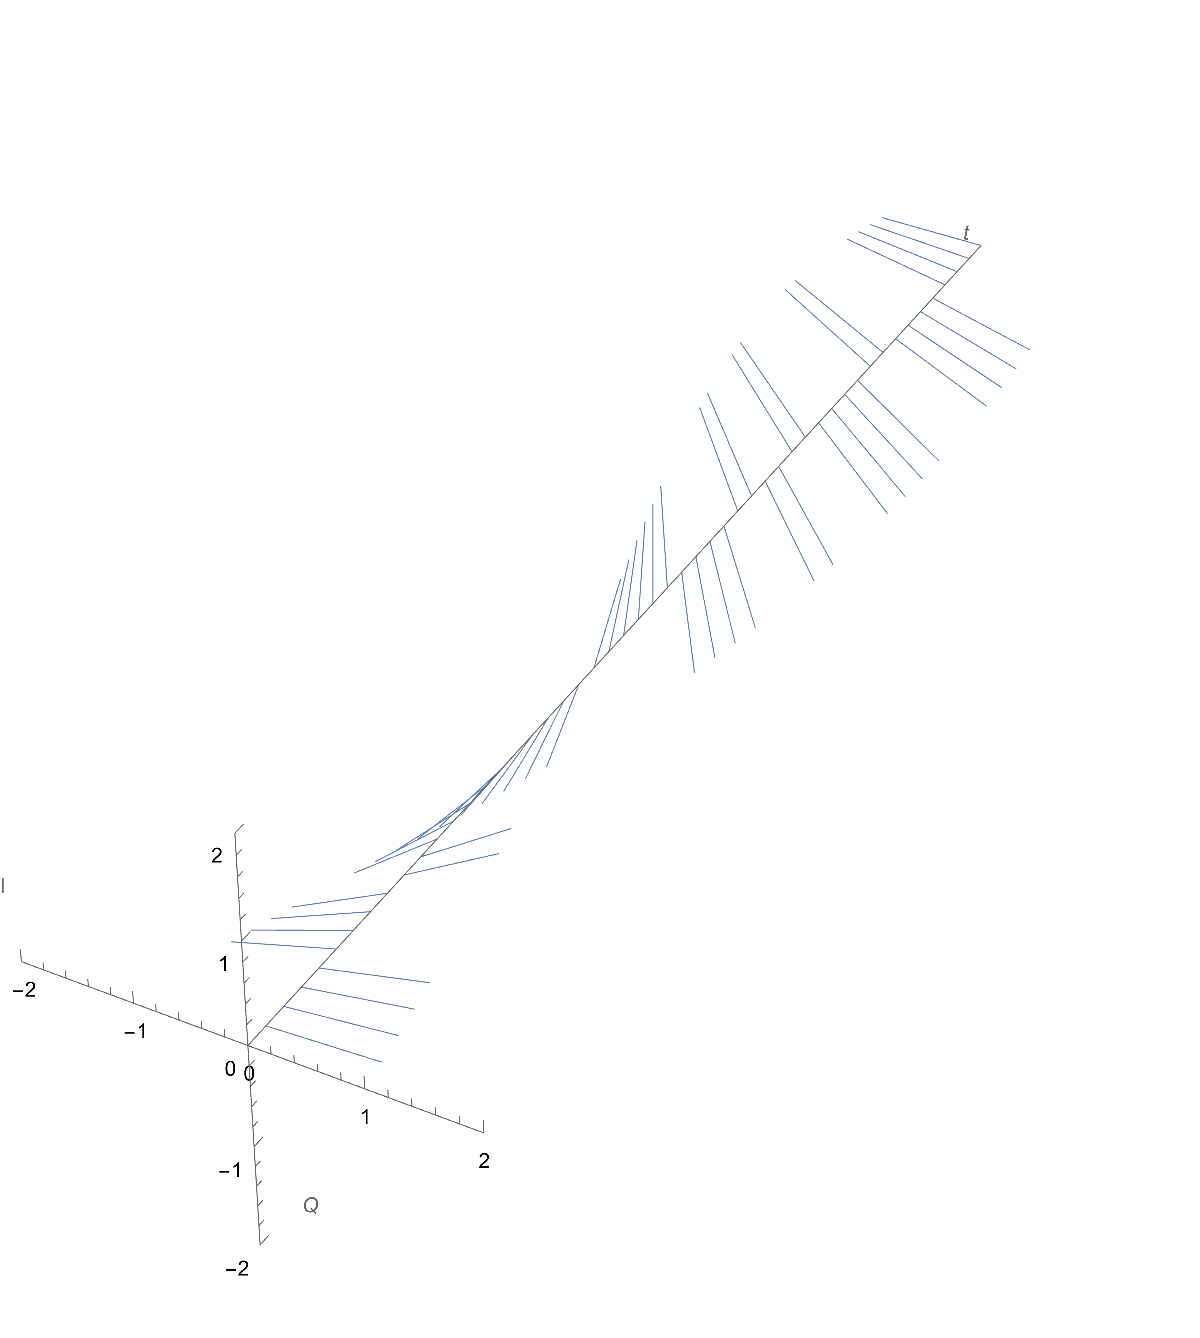
\includegraphics[width=\textwidth * 2 / 5]{1 frequency shifted.pdf} \raisebox{2.75cm}{\Large $\Rightarrow$} \qquad 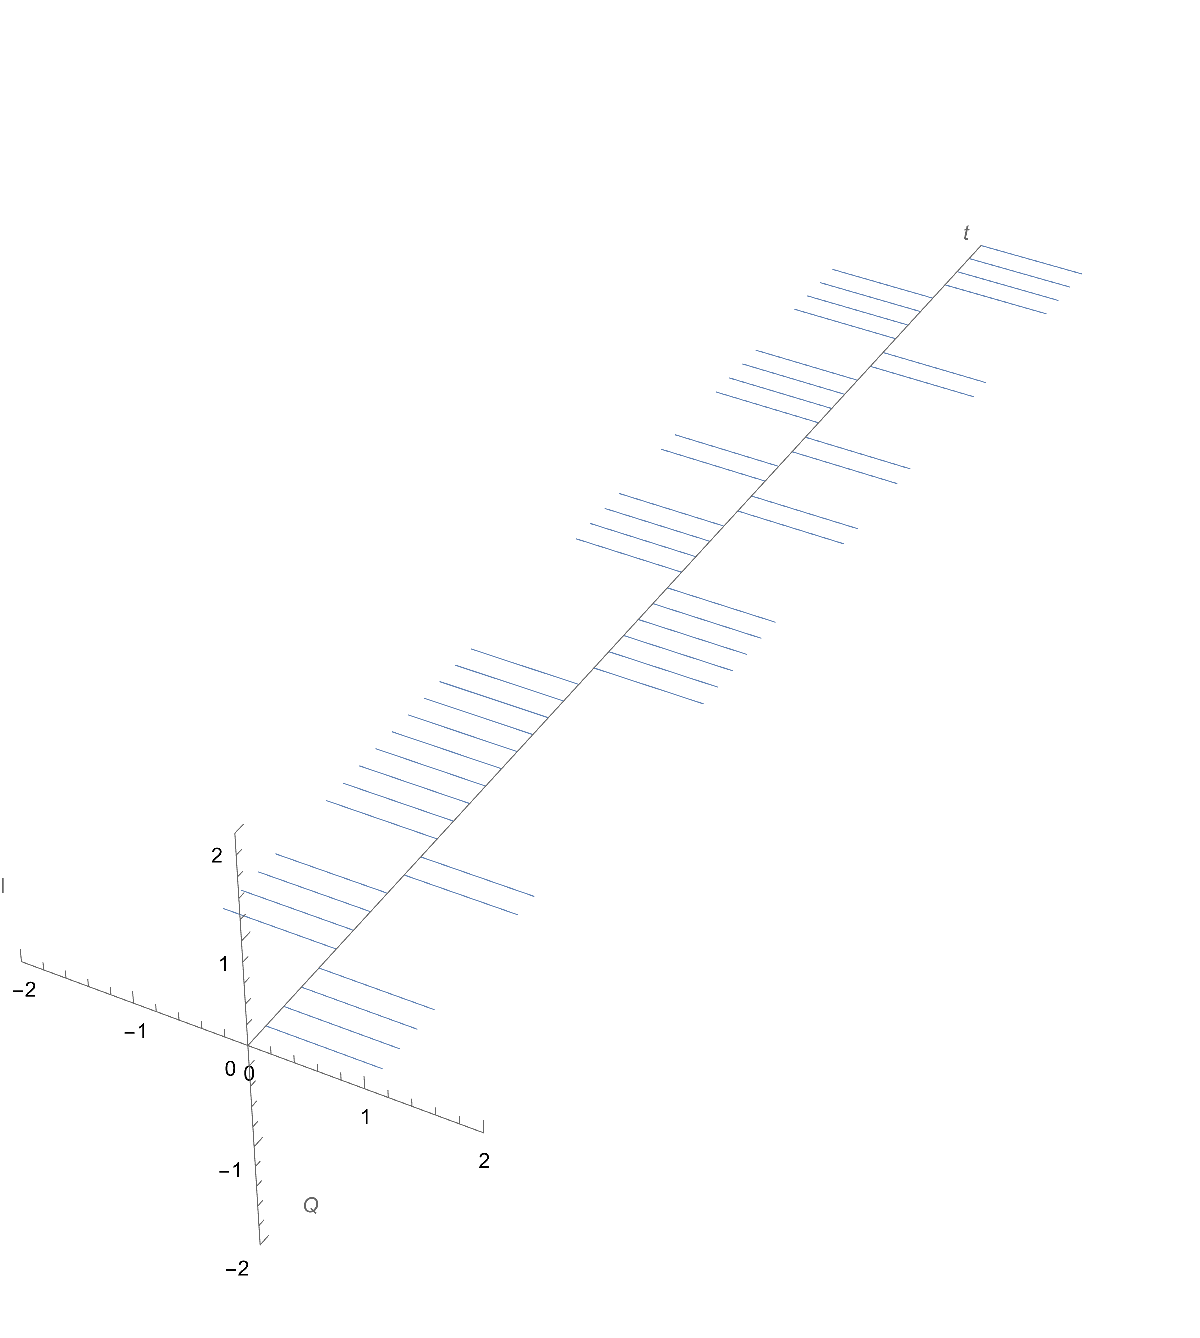
\includegraphics[width=\textwidth * 2 / 5]{2 post carrier wipeoff.pdf}}
\end{frame}

\begin{frame}
    \frametitle{Carrier wipeoff}

    \centering
    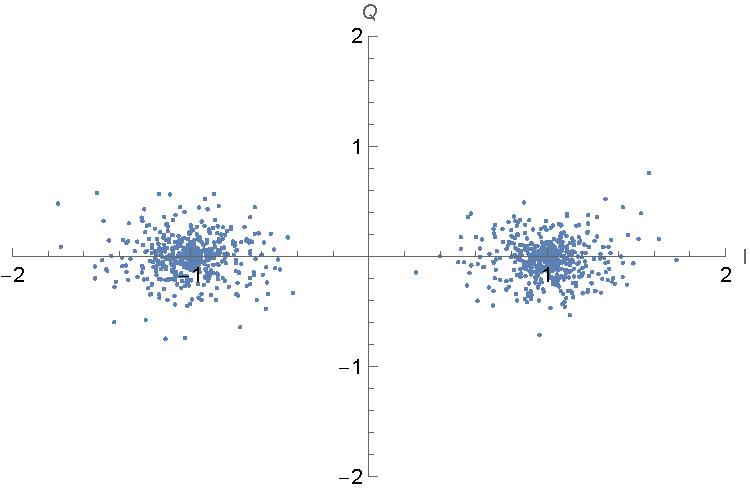
\includegraphics[width=\textwidth * 3 / 5]{3 correlations.pdf}
\end{frame}

\begin{frame}
    \frametitle{Carrier wipeoff}

    \centering
    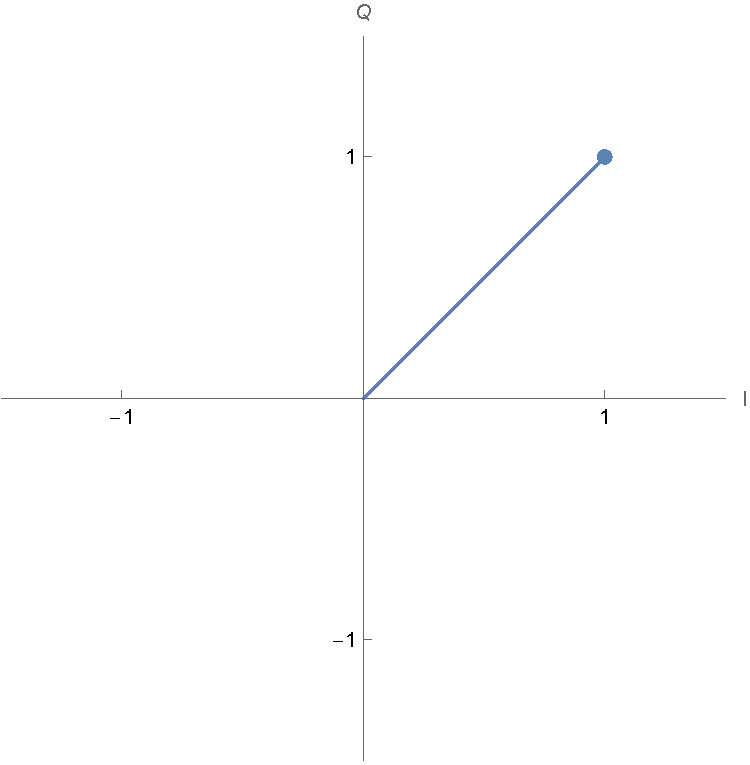
\includegraphics[width=\textwidth / 3]{4 bit ambiguity.pdf}
\end{frame}

\section{PRN code tracking}

\begin{frame}
    \frametitle{Delay-locked loop}

    \only<1>{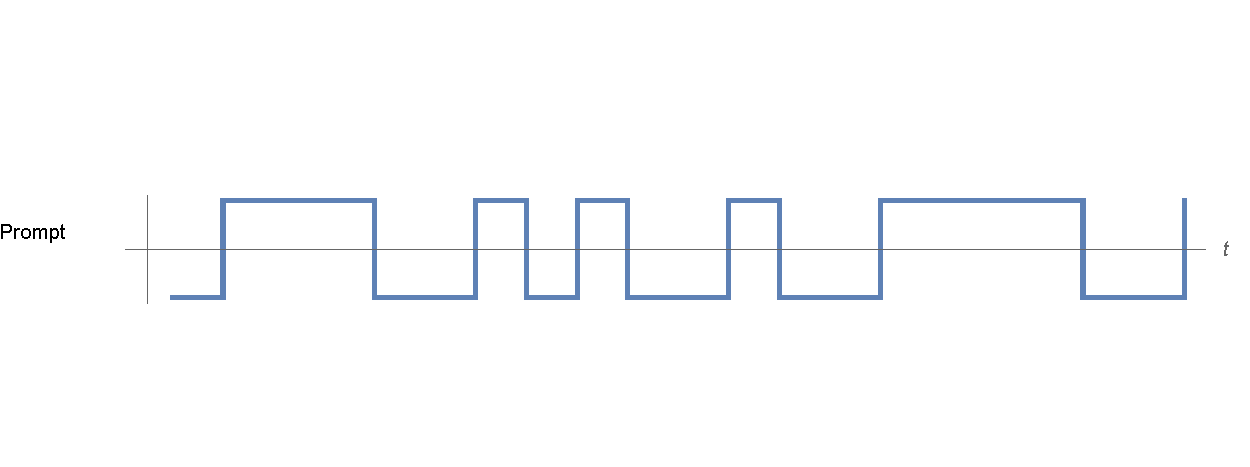
\includegraphics[width=\textwidth]{5 prompt.pdf}}%
    \only<2>{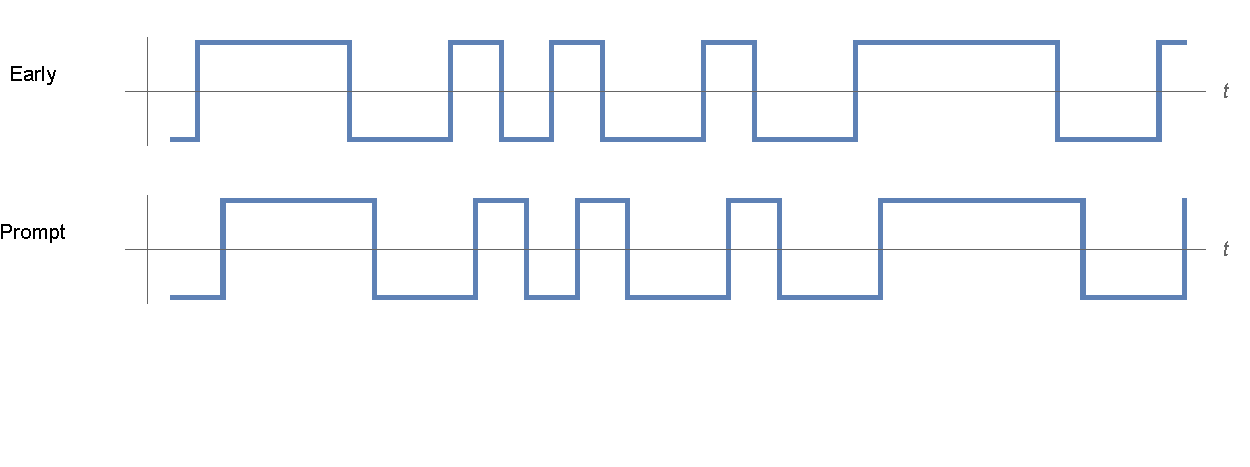
\includegraphics[width=\textwidth]{6 prompt early.pdf}}%
    \only<3>{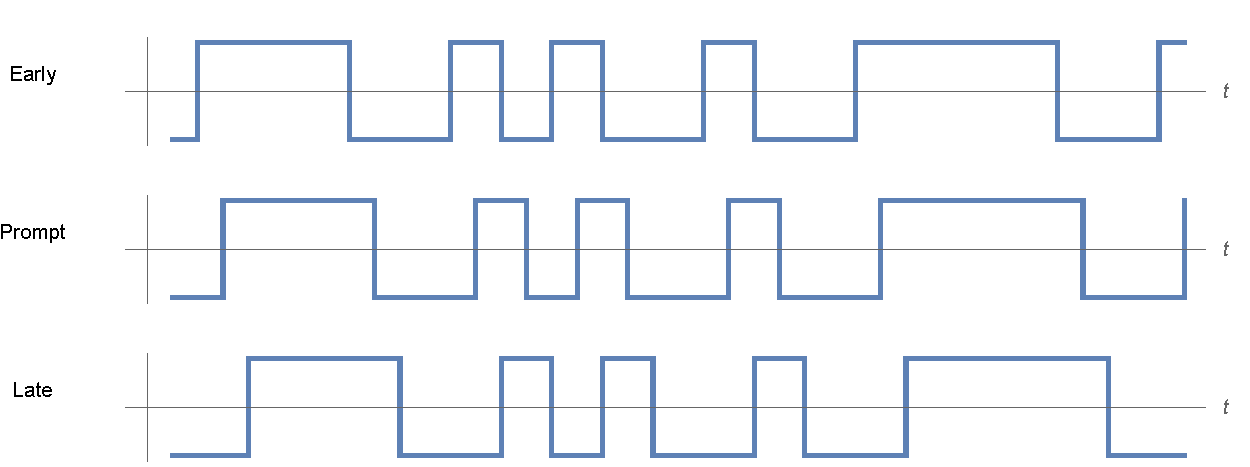
\includegraphics[width=\textwidth]{7 prompt early late.pdf}}
\end{frame}

\begin{frame}
    \frametitle{Accounting for frequency shift}

    \only<1>{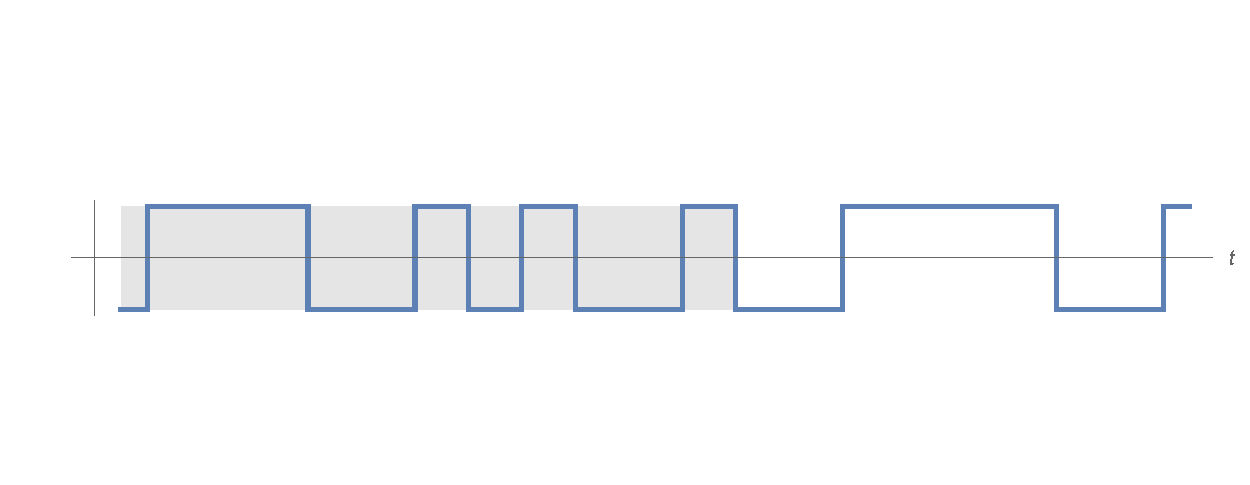
\includegraphics[width=\textwidth]{8 no frequency shift.pdf}}%
    \only<2>{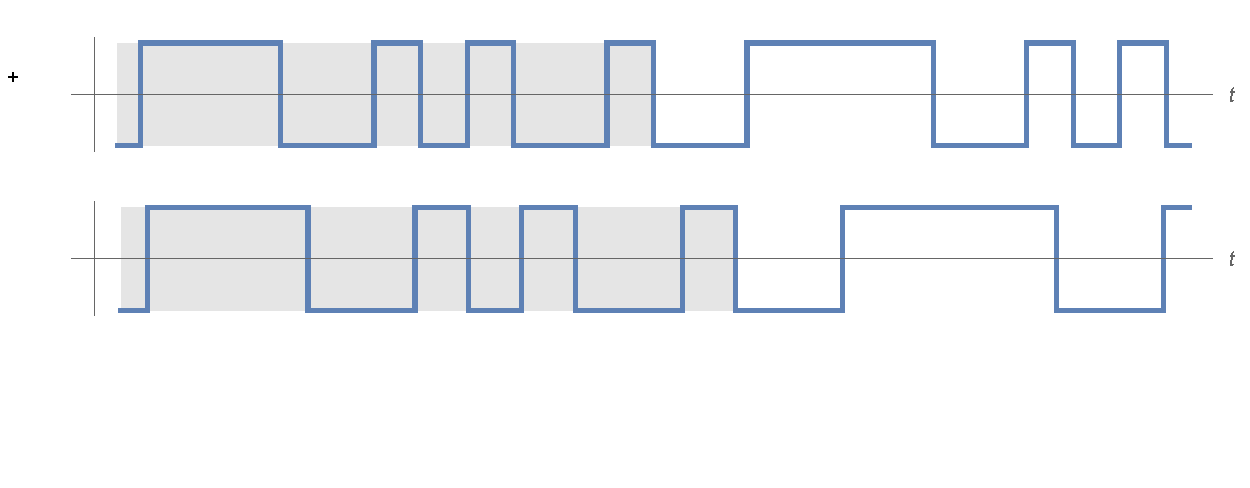
\includegraphics[width=\textwidth]{9 positive.pdf}}%
    \only<3>{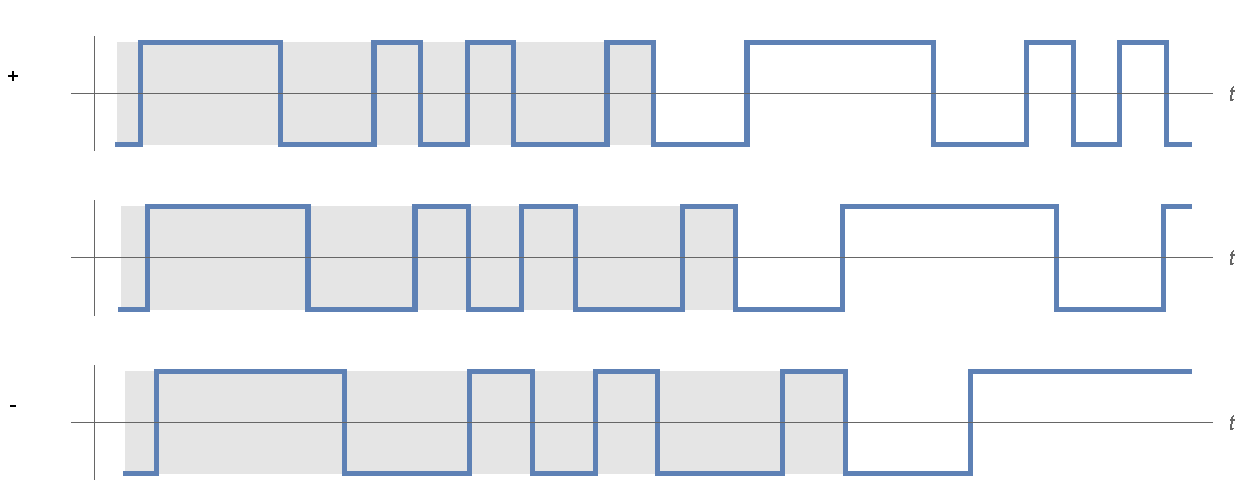
\includegraphics[width=\textwidth]{10 positive and negative.pdf}}
\end{frame}

\begin{frame}
    \frametitle{Accounting for frequency shift}

    \centering
    \Large
    \[\Delta \phi = \overbrace{2046}^{\mathclap{\text{PRN length}}} \times \underbrace{\Delta f \div f_{L1}}_{\mathclap{\text{Percentage frequency change}}}\]
\end{frame}

\section{Correlation}

\begin{frame}
    \frametitle{Correlation}

    \begin{center}
        \only<1>{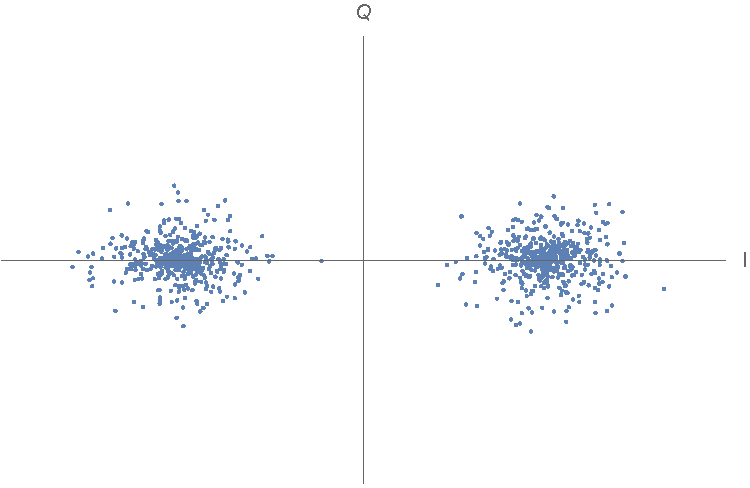
\includegraphics[width=\textwidth / 2]{11 correlations.pdf}}%
        \only<2->{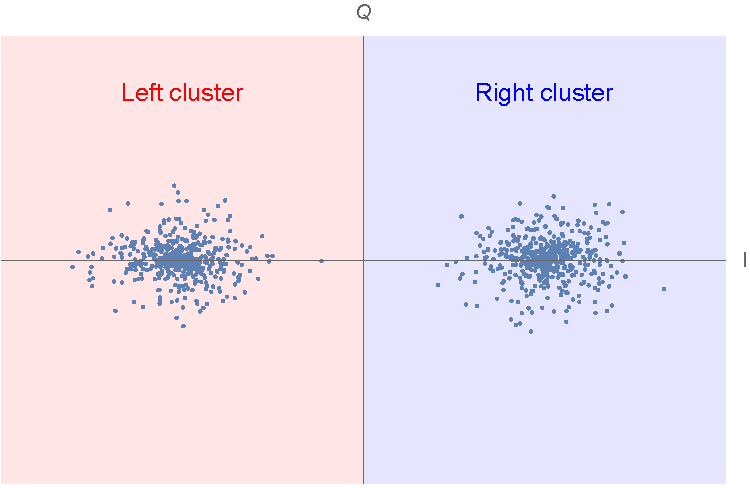
\includegraphics[width=\textwidth / 2]{12 correlations with regions.pdf}}
    \end{center}

    \begin{itemize}
        \item<3-> These fragments are called ``pseudosymbols''
    \end{itemize}
\end{frame}

\section{Carrier wave tracking}

\begin{frame}
    \frametitle{Carrier wave tracking}

    \begin{itemize}
        \item Update our estimates of the carrier wave's frequency shift and phase
        
        \item<2-> Use a phase-locked loop (Costas loop)
        
        \begin{itemize}
            \item<3-> Calculate a single value that represents the error in both estimates

            \item<4-> Use it to update them
        \end{itemize}
    \end{itemize}
\end{frame}

\begin{frame}
    \frametitle{Carrier wave tracking}

    \centering
    \only<1>{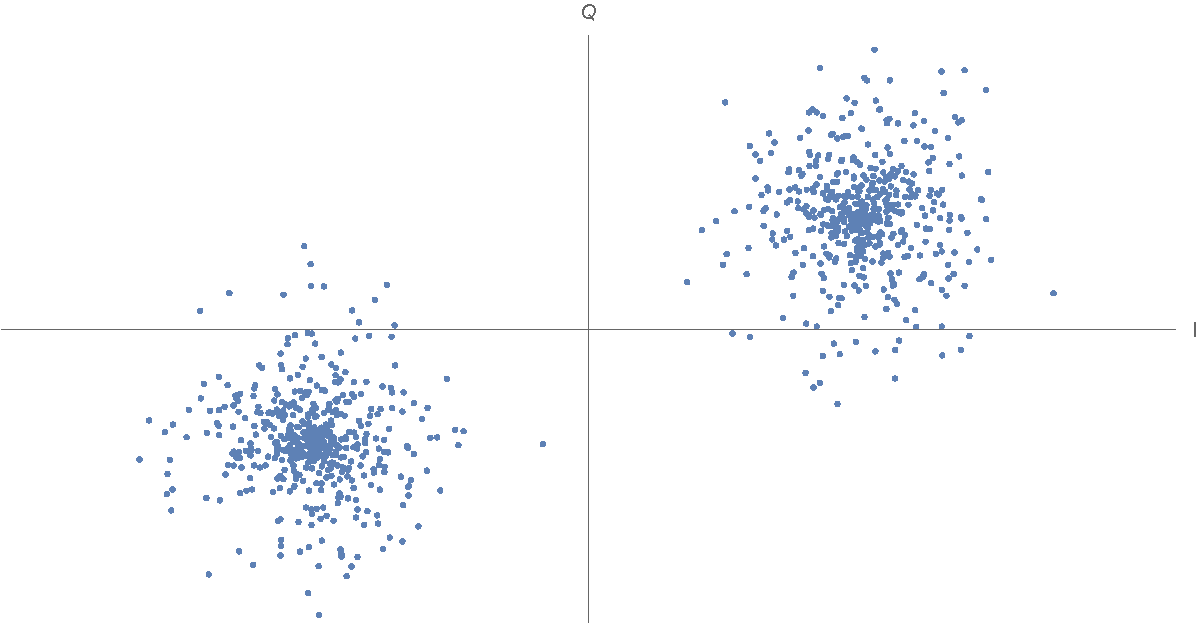
\includegraphics[width=\textwidth * 3 / 4]{13 clusters.pdf}}%
    \only<2>{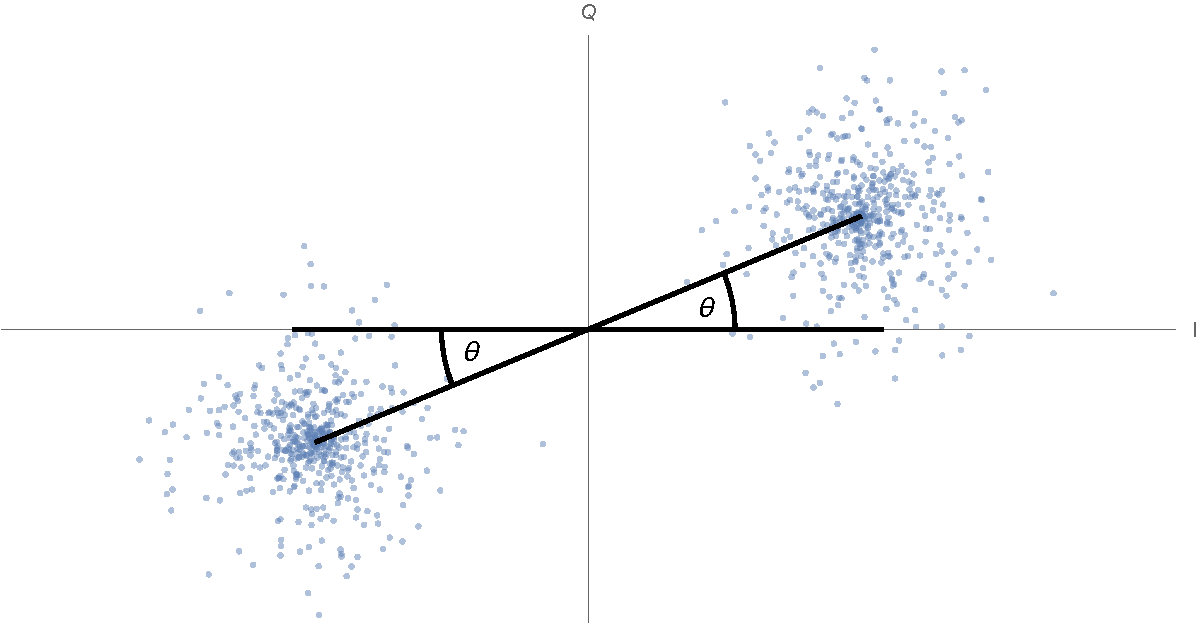
\includegraphics[width=\textwidth * 3 / 4]{14 cluster angles.pdf}}%
    \only<3->{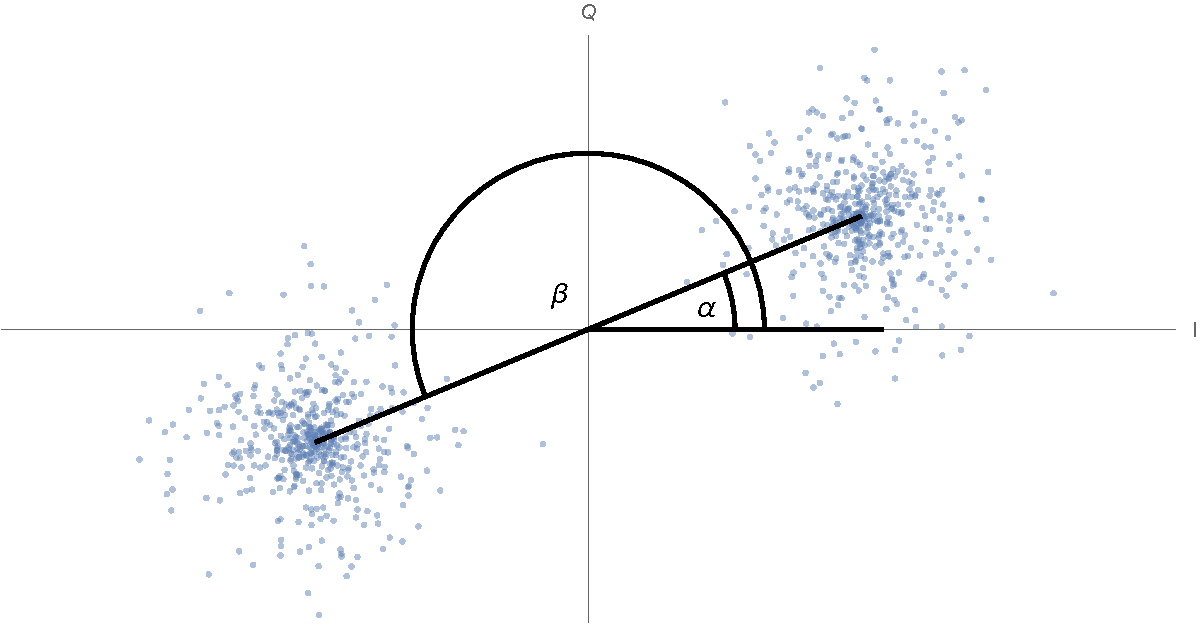
\includegraphics[width=\textwidth * 3 / 4]{15 cluster angles 2.pdf}}%

    \begin{itemize}
        \item<4-> Use \texttt{atan} rather than \texttt{atan2}
    \end{itemize}
\end{frame}

\begin{frame}
    \frametitle{Carrier wave tracking}

    \begin{itemize}
        \item<2-> Each estimate has an associated gain factor
        
        \item<3-> To update an estimate:

        \begin{enumerate}
            \item<4-> Calculate \texttt{error $\times$ gain}

            \item<5-> Subtract it from the current estimate
        \end{enumerate}

        \item<6-> Determine gain factors experimentally
        
        \item<7-> Phase gain should be around 25 $\times$ the frequency shift gain
    \end{itemize}
\end{frame}

\begin{frame}
    \frametitle{Recap}

    \begin{itemize}
        \item<2-> Negate rotation of samples caused by frequency shift and phase (carrier wipeoff)
        
        \item<3-> Update PRN code phase using a delay-locked loop
        
        \begin{enumerate}
            \item<4-> Generate early and late replicas of the PRN code
            
            \item<5-> Calculate their correlation with the $\qty{1}{ms}$ of samples

            \item<6-> Compare the magnitudes of correlations to determine best alignment
            
            \item<7-> Update the estimate
        \end{enumerate}

        \item<8-> Calculate the correlation of the samples and the PRN code $\Rightarrow$ pseudosymbol
        
        \item<9-> Update carrier wave frequency shift and phase using a phase-locked loop (Costas loop)
        
        \begin{enumerate}
            \item<10-> Calculate error as angle of correlation

            \item<11-> Multiply error by each estimate's gain factor

            \item<12-> Subtract the result from each estimate
        \end{enumerate}
    \end{itemize}
\end{frame}

\end{document}